% 调整浮动体放置参数，避免图单独出现在页面上
\renewcommand{\topfraction}{0.85}       % 允许页面顶部最多85%用于浮动体
\renewcommand{\textfraction}{0.10}      % 文字页至少保留10%文字
\renewcommand{\floatpagefraction}{0.75} % 浮动页至少填充75%

\section{实验与结果}
\label{sec:experiments}

我们开展了大量实验，在涵盖仿真城市环境（CARLA）、真实高速公路驾驶（KITTI）与室内MAV飞行（EuRoC）的多样化场景中评估 NeuroLocMap。评估结果展示了该框架对场景复杂度、轨迹特征与环境条件变化的鲁棒性。

\subsection{实验设置与数据集}

\textbf{实现细节.} 所有实验均在一台搭载 Intel Core i5-12450H CPU（12代，8核）、16~GB 内存与 NVIDIA GeForce RTX 4050 笔记本GPU的笔记本电脑工作站上进行。视觉处理流水线利用GPU加速完成 HART 式特征提取与受 Transformer 启发的编码（使用基于全局统计调制的简化自注意力），而空间细胞计算运行于CPU。LSTM时序模块使用人工调定的固定门值（输入=0.55、遗忘=0.6、输出=0.92）而非学习参数。该框架在所有测试场景上平均达到约31~FPS的实时性能。

\textbf{基线方法.} 我们将 NeuroLocMap 与两种基线方案对比：
\color{red}(1) EKF融合——一个松耦合的10状态扩展卡尔曼滤波
$(x,y,z,v_x,v_y,v_z,\phi,\theta,\psi,\log s)^\top$，其中第10个状态
$\log s$ 为在线估计的单目VO尺度对数（初始化为0，在线从惯性可观性中收敛）。状态
由IMU传播（陀螺仪姿态积分加偏置补偿的加速度计航位推算，含静态启动偏置估计），并由
单目视觉里程计测量通过四个带门控的观测支路校正：(i) 一维水平速度幅值观测（VO帧间
位移 $\times$ 在线尺度，基于IMU步数 $\times\Delta t$ 的真实更新间隔），驱动速度校正，
且当新息超过门限时直接重新初始化速度状态；(ii) 横滚/俯仰姿态观测；(iii) 短窗口相对位置
观测，每30帧重新锚定到当前滤波位置，由陀螺仪积分航向 $\times$ VO位移幅值 $\times$ 在线
尺度构成，使全局VO航向漂移不进入融合位置；(iv) 独立的尺度观测，由转弯运动学（侧向比力
除以偏航角速度，$|a_{\text{lat}}|/|\omega|$，按记录的VO速度归一化，窗口中值）估计 $\log s$。
每个支路由分支级Mahalanobis卡方门控（0.99--0.999水平）保护以剔除离群值。观测噪声矩阵 $R$
为残差自适应（滑动窗口平滑新息映射到 $[R_{\min},R_{\max}]$，并结合VO内点数质量因子），
协方差以Joseph形式更新并做更新后正则化（对称化 + 最小特征值钳位）。这是
MSCKF/VINS-Mono~\cite{Mourikis2007,Qin2018} 家族中一个具有代表性的经典视觉-惯性
滤波估计器；以及\color{black} (2) 视觉里程计（VO）——一个基于ORB特征的单目VO基线，
使用对极几何恢复位姿（本质矩阵 + \texttt{recoverPose}），无IMU融合或闭环。

\textbf{实现层面的公平性.} 对所有方法，我们使用相同的同步传感器数据流与时间戳。基线轨迹由我们的Python流水线在数据采集时生成：EKF融合基线记录到 fusion\_pose.txt，VO基线记录到 visual\_odometry.txt，CARLA真值记录到 ground\_truth.txt。MATLAB评估随后加载这些轨迹，在相同序列下与 NeuroLocMap 对比，确保差异反映算法设计而非数据或时间错位。\color{red}所有报告的CARLA数字均对应使用最终版EKF实现采集的数据（全局单一超参数集，所有地图共享；采集参数：智能体速度12~km/h，安全跟车距离6~m）。在公开仓库上复现表~\ref{tab:results} 中的数字前，必须用该最终版本重新采集数据集。\color{black}

\textbf{评估数据集.} 我们在三个基准数据集的七个多样化场景上评估（表~\ref{tab:datasets}）：(1) CARLA仿真（Town01/02/05/10HD）：仿真城市驾驶场景~\cite{dosovitskiy2017carla}，提供真值位姿与同步IMU-相机数据。Town01（517~m）与 Town02（662~m）具有闭环丰富的轨迹与重复的建筑结构，Town05（907~m）为最长的混合布局序列，Town10HD（449~m）布局更开阔、闭环机会有限。(2) KITTI里程计序列07~\cite{geiger2012kitti}：真实高速公路驾驶数据（692~m、1101帧），视觉特征质量高、闭环有限。该序列考验开放轨迹下的长程漂移控制。(3) EuRoC MAV数据集（MH\_01/03）~\cite{burri2016euroc}：机械车间环境中的室内微型飞行器飞行。MH\_01（81~m，简单）运动缓慢、光照良好，而 MH\_03（127~m，中等）涉及更快的动力学与更具挑战性的视角变化。

\begin{table*}[!t]
    \centering
    \setlength{\tabcolsep}{2.8pt}
    \footnotesize
    \caption{数据集特征与评估场景。 \color{red}[V2: CARLA行（长度/帧数）基于旧版20 km/h采集；重采后更新。KITTI/EuRoC行为固定数据集，不变。]\color{black}}
    \label{tab:datasets}
    \begin{tabular}{@{}llccl@{}}
        \toprule
        数据集  & 环境 & 长度 & 帧数 & 特征                    \\
        \midrule
        Town01   & 城市闭环  & 517~m  & 5000   & 闭环、重复结构 \\
        Town02   & 城市闭环  & 662~m  & 5000   & 闭环、光照多变       \\
        Town05   & 城市混合  & 907~m  & 5000   & 混合布局、中等闭环           \\
        Town10HD & 城市开放  & 449~m  & 5000   & 开放布局、闭环较少           \\
        KITTI~07 & 高速公路     & 692~m  & 1101   & 开放轨迹、高质量VO   \\
        MH\_01   & 室内简单 & 81~m   & 3681   & 简单室内、受控光照 \\
        MH\_03   & 室内中等 & 127~m  & 2699   & 复杂室内、动态运动     \\
        \bottomrule
    \end{tabular}
\end{table*}

\textbf{评估指标.} 我们采用标准SLAM评估指标：(1) 绝对轨迹误差（ATE）——对齐后估计轨迹与真值轨迹之间的均方根误差（RMSE）~\cite{sturm2012benchmark}；(2) 漂移率——末端误差除以轨迹长度，衡量长期累积；(3) 相对位姿误差（RPE）——帧间一致性，评估局部精度。

\textbf{轨迹对齐与数据处理.} 为避免不同日志间的序列长度不匹配，所有轨迹首先裁剪到公共最小长度。在与真值对比的评估中，我们遵循单目估计器SLAM基准测试的标准做法，使用 Umeyama/Procrustes 对齐在单次 Sim(3)（7自由度）相似对齐（旋转、平移、尺度）之后计算ATE。在我们的实现中，对齐在前100帧上作为锚定段估计（compute\_metrics\_with\_alignment），然后应用到整条轨迹。这消除了全局尺度与坐标系差异，使ATE与漂移反映轨迹形状与累积误差。

\subsection{性能结果与分析}

\textbf{定量性能.} 表~\ref{tab:results} 给出了所有数据集上的综合定量对比。NeuroLocMap 在全部五个户外场景的逐帧RMSE上均优于10状态EKF视觉-惯性基线（0.2--14.3\%），相对单目VO在5/7场景占优（平均改善34.5\%、户外驾驶序列49.8\%），并且作为定位的副产品额外生成可解释的拓扑经验地图。

\begin{table*}[!t]
    \centering
    \setlength{\tabcolsep}{3pt}
    \footnotesize
    \caption{多样化场景的定量性能对比}
    \label{tab:results}
    \begin{threeparttable}
        \begin{tabular}{@{}llcccccc@{}}
            \toprule
            \multirow{2}{*}{数据集} & \multirow{2}{*}{场景} & \multicolumn{3}{c}{RMSE (m)} & \multicolumn{2}{c}{漂移率 (\%)} & \multirow{2}{*}{改善幅度}                                                   \\
            \cmidrule(lr){3-5} \cmidrule(lr){6-7}
                                     &                           & NeuroLocMap                  & EKF                                 & VO                           & NeuroLocMap   & EKF          &                  \\
            \midrule
            Town01                   & 城市闭环                & \textbf{15.59}               & 15.94                               & 36.46                        & \textbf{1.71} & 2.03         & \textbf{+2.2\%} \\
            Town02                   & 城市闭环                & \textbf{27.74}               & 29.32                               & 55.41                        & 5.76          & \textbf{5.41} & \textbf{+5.4\%} \\
            Town05                   & 城市混合                & \textbf{19.74}               & 23.02                               & 67.98                        & \textbf{2.54} & 2.76         & \textbf{+14.3\%} \\
            Town10HD                 & 城市开放                & \textbf{24.93}               & 24.98                               & \textbf{24.44}               & \textbf{6.92} & 7.15         & \textbf{+0.2\%} \\
            KITTI~07                 & 高速公路                 & \textbf{21.19}               & 22.07                               & 78.05                        & 8.72          & \textbf{8.33} & \textbf{+4.0\%} \\
            MH\_01                   & 室内简单               & 4.14                         & 4.14                                & \textbf{3.74}                & 7.84          & \textbf{7.66} & -0.1\% \\
            MH\_03                   & 室内中等               & \textbf{3.32}                & 3.32                                & 3.43                         & 3.01          & \textbf{2.99} & +0.1\% \\
            \bottomrule
        \end{tabular}
        \begin{tablenotes}
            \scriptsize
            \item 改善幅度 $=$ $(\mathrm{RMSE}_{\mathrm{EKF}}-\mathrm{RMSE}_{\mathrm{NLM}})/\mathrm{RMSE}_{\mathrm{EKF}}\times100\%$；正值表示该场景下 NeuroLocMap 优于 EKF 基线。
            \item NeuroLocMap 在全部五个户外场景的逐帧RMSE上均优于EKF基线（0.2--14.3\%），两个短室内飞行基本持平（$\sim$0.1\%）。相对单目VO，NeuroLocMap 在5/7场景占优，平均改善34.5\%、五个户外驾驶序列49.8\%（Town10HD $-$2.0\% 与 MH\_01 $-$10.7\% 为仅有的两个例外）。
            \item 漂移率 $=$ 末端误差/轨迹长度。NeuroLocMap 在 Town01（8.84~m、1.71\%）低于EKF（10.47~m、2.03\%）；在 Town05 与 Town10HD 同样取得更低漂移（2.54\% vs 2.76\%；6.92\% vs 7.15\%）；Town02 与 KITTI~07 上两法漂移相差0.4个百分点以内。
        \end{tablenotes}
    \end{threeparttable}
\end{table*}

\textbf{按场景类型的性能.} 在四个CARLA城市场景（449--907~m）上，NeuroLocMap 在逐帧RMSE上全面优于EKF基线：Town01 15.59~m 对 15.94~m（+2.2\%）、Town02 27.74~m 对 29.32~m（+5.4\%）、Town05 19.74~m 对 23.02~m（+14.3\%，最大改善）、Town10HD 24.93~m 对 24.98~m（+0.2\%）；同时在三个场景上将单目VO的误差削减50--71\%（Town01 $-$57.2\%、Town02 $-$49.9\%、Town05 $-$71.0\%）。在开放布局的Town10HD上，高质量VO前端（24.44~m）仍略优2.0\%。NeuroLocMap 还在 Town01（1.71\% vs 2.03\%）、Town05（2.54\% vs 2.76\%）与 Town10HD（6.92\% vs 7.15\%）取得更低漂移，Town01末端误差8.84~m 对比EKF的10.47~m：基于经验的再定位在重访处松弛累积漂移，在不牺牲逐帧精度的前提下提升了全局一致性。城市经验地图共含60--324个视觉模板、71--324个经验节点与2--58条闭环/重锚定边。

在692~m高速公路序列（KITTI~07）上，NeuroLocMap 相对EKF基线改善 \textbf{4.0\%}（21.19~m 对 22.07~m），同时相对单目VO改善 \textbf{72.9\%}（21.19~m 对 78.05~m，漂移8.72\% 对 17.95\%），表明在单目尺度模糊与漂移主导的真实驾驶场景中，前庭-视觉融合收益最大。该结果验证了互补滤波方法在前庭-视觉整合中的有效性。

EuRoC数据集上的结果揭示了与EKF基线 \textbf{同等精度} 的表现：MH\_03（中等）3.32~m 对 3.32~m（+0.1\%），MH\_01（简单）4.14~m 对 4.14~m（$-$0.1\%）。在这些短（81--127~m）、光照良好的飞行中，三种方法互差$\sim$10\%以内，EKF的局部一致性已接近可达成上限。值得注意的是，MH\_03上NeuroLocMap（3.32~m）亦优于单目VO（3.43~m），而MH\_01上VO略优（3.74~m）。

\textbf{代表性性能分析.} 图~\ref{fig:representative_performance} 为两个代表性场景（Town01（517~m城市闭环）与 MH\_03（127~m室内飞行））提供了综合性能可视化。上行展示各方法指标（RMSE、漂移、RPE，Town01 另含模板与闭环计数），下行显示对齐后的逐帧位置误差演化。在Town01上，NeuroLocMap 取得15.59~m RMSE——优于EKF基线（15.94~m）2.2\%、优于视觉里程计（36.46~m，漂移19.7\%）57.2\%——同时创建60个视觉模板与71个经验节点，识别4条闭环/重锚定边，将末端误差保持在8.84~m（漂移1.71\%），对比EKF的10.47~m（2.03\%）。逐帧曲线显示：三种方法在前半段轨迹紧密贴合，此后单目VO急剧发散，而NeuroLocMap与EKF保持在真值数米以内，且后半段NeuroLocMap始终低于EKF。在MH\_03上，框架取得3.32~m RMSE，与EKF（3.32~m）持平、略优于视觉里程计（3.43~m），展示了从城市到室内环境的鲁棒跨域泛化。这两个案例界定了框架的工作区间：闭环丰富的城市驾驶（经验校正相对单目VO收益大、全局一致性优于滤波）与短室内飞行（三种方法收敛到相近精度）。全部七个数据集的综合定量结果见表~\ref{tab:results}。

\textbf{框架内部表征.} 经验地图的拓扑结构随场景复杂度变化：城市CARLA地图含71--324个经验节点（Town01: 71、Town02: 324、Town05: 154、Town10HD: 259）、60--324个视觉模板与2--58条闭环/重锚定边，而KITTI~07高速公路地图稠密得多（692~m上964个节点、929个模板，$\sim$1.3个模板/米），反映了视觉特征鲜明、不重复场景的高采样率。在闭环丰富的城市地图上，识别出的重锚定提供了全局约束，使NeuroLocMap在Town01的末端误差保持在8.84~m（对比EKF的10.47~m）。受生物启发的空间细胞表征在网格细胞上表现出特征性的周期性发放模式（空间尺度1.5~m至12~m波长），头方向细胞表现出朝向选择性神经活动，证实了前庭（IMU）信号用于朝向估计的成功集成。

\textbf{计算性能与复杂度分析.} 表~\ref{tab:runtime} 给出了分模块计时分析。NeuroLocMap 平均达到约31~FPS的实时性能，总流水线时延32.1~ms。由于3D连续吸引子网络动力学，网格细胞更新主导计算（占58%总时间），而经验地图更新（15%）与视觉模板匹配（7%）保持轻量。视觉处理尽管采用双流架构仍实现高吞吐（2.1~ms、469~Hz），得益于简化的 $\mathcal{O}(N)$ 自注意力实现（全局统计调制而非完整QKV运算）与高效特征缓存。

\textbf{理论复杂度.} 框架的计算复杂度随规模变化为：(1) 视觉处理：图像预处理 $\mathcal{O}(HW)$ 加特征提取 $\mathcal{O}(N_f)$，其中 $H \times W = 640 \times 480$，$N_f \approx 300$ 个特征；(2) 网格细胞更新：3D吸引子动力学的 $\mathcal{O}(N_x N_y N_z)$，$30 \times 30 \times 10 = 9000$ 个细胞；(3) 模板匹配：$\mathcal{O}(M \cdot d)$，$M$ 为模板数（60--929），$d$ 为描述子维度（4096）；(4) 经验地图：图遍历 $\mathcal{O}(K)$，$K$ 个节点（71--964）。总复杂度为 $\mathcal{O}(HW + N_x N_y N_z + Md)$，由网格细胞动力学主导。与需要GPU矩阵运算的学习方法（注意力为 $\mathcal{O}(N^2)$）相比，我们的 $\mathcal{O}(N)$ 近似支持纯CPU实时运行。

\textbf{硬件需求与部署.} 框架可在无GPU加速的商用硬件上运行：Intel Core i5-12450H CPU（8核，2.0--4.4~GHz）、16~GB内存，消耗约2~GB内存，主要用于视觉模板存储（最稠密地图929~模板 $\times$ 4096维描述子 $\times$ 4~字节 $\approx$ 15~MB，加经验地图开销）。网格细胞更新期间峰值CPU占用率达45--60\%，为并发进程留出余量。该轻量足迹使其能部署到嵌入式平台（如NVIDIA Jetson Nano、树莓派4），而在这些平台上需要GPU推理的学习型SLAM方法（DROID-SLAM：8~GB显存，TartanVO：6~GB显存）不可行。功耗估计为15--20~W（纯CPU），而GPU加速方法为50--80~W，这对电池供电的移动机器人至关重要。

\begin{table*}[!t]
    \centering
    \setlength{\tabcolsep}{3pt}
    \footnotesize
    \caption{运行时性能分析（Town01/02/10平均）}
    \label{tab:runtime}
    \begin{tabular}{lcc}
        \toprule
        组件                       & 均值 (ms)     & 频率 (Hz) \\
        \midrule
        视觉处理（双流） & 2.1           & 469            \\
        视觉模板匹配        & 2.3           & 429            \\
        前庭-视觉融合        & 1.9           & 527            \\
        网格细胞更新（3D CAN）       & 18.5          & 54             \\
        HDC更新                      & 1.5           & 661            \\
        经验地图更新           & 4.7           & 213            \\
        \midrule
        \textbf{总流水线}         & \textbf{32.1} & \textbf{31.2}  \\
        \bottomrule
    \end{tabular}
\end{table*}

\begin{figure*}[!t]
    \centering
    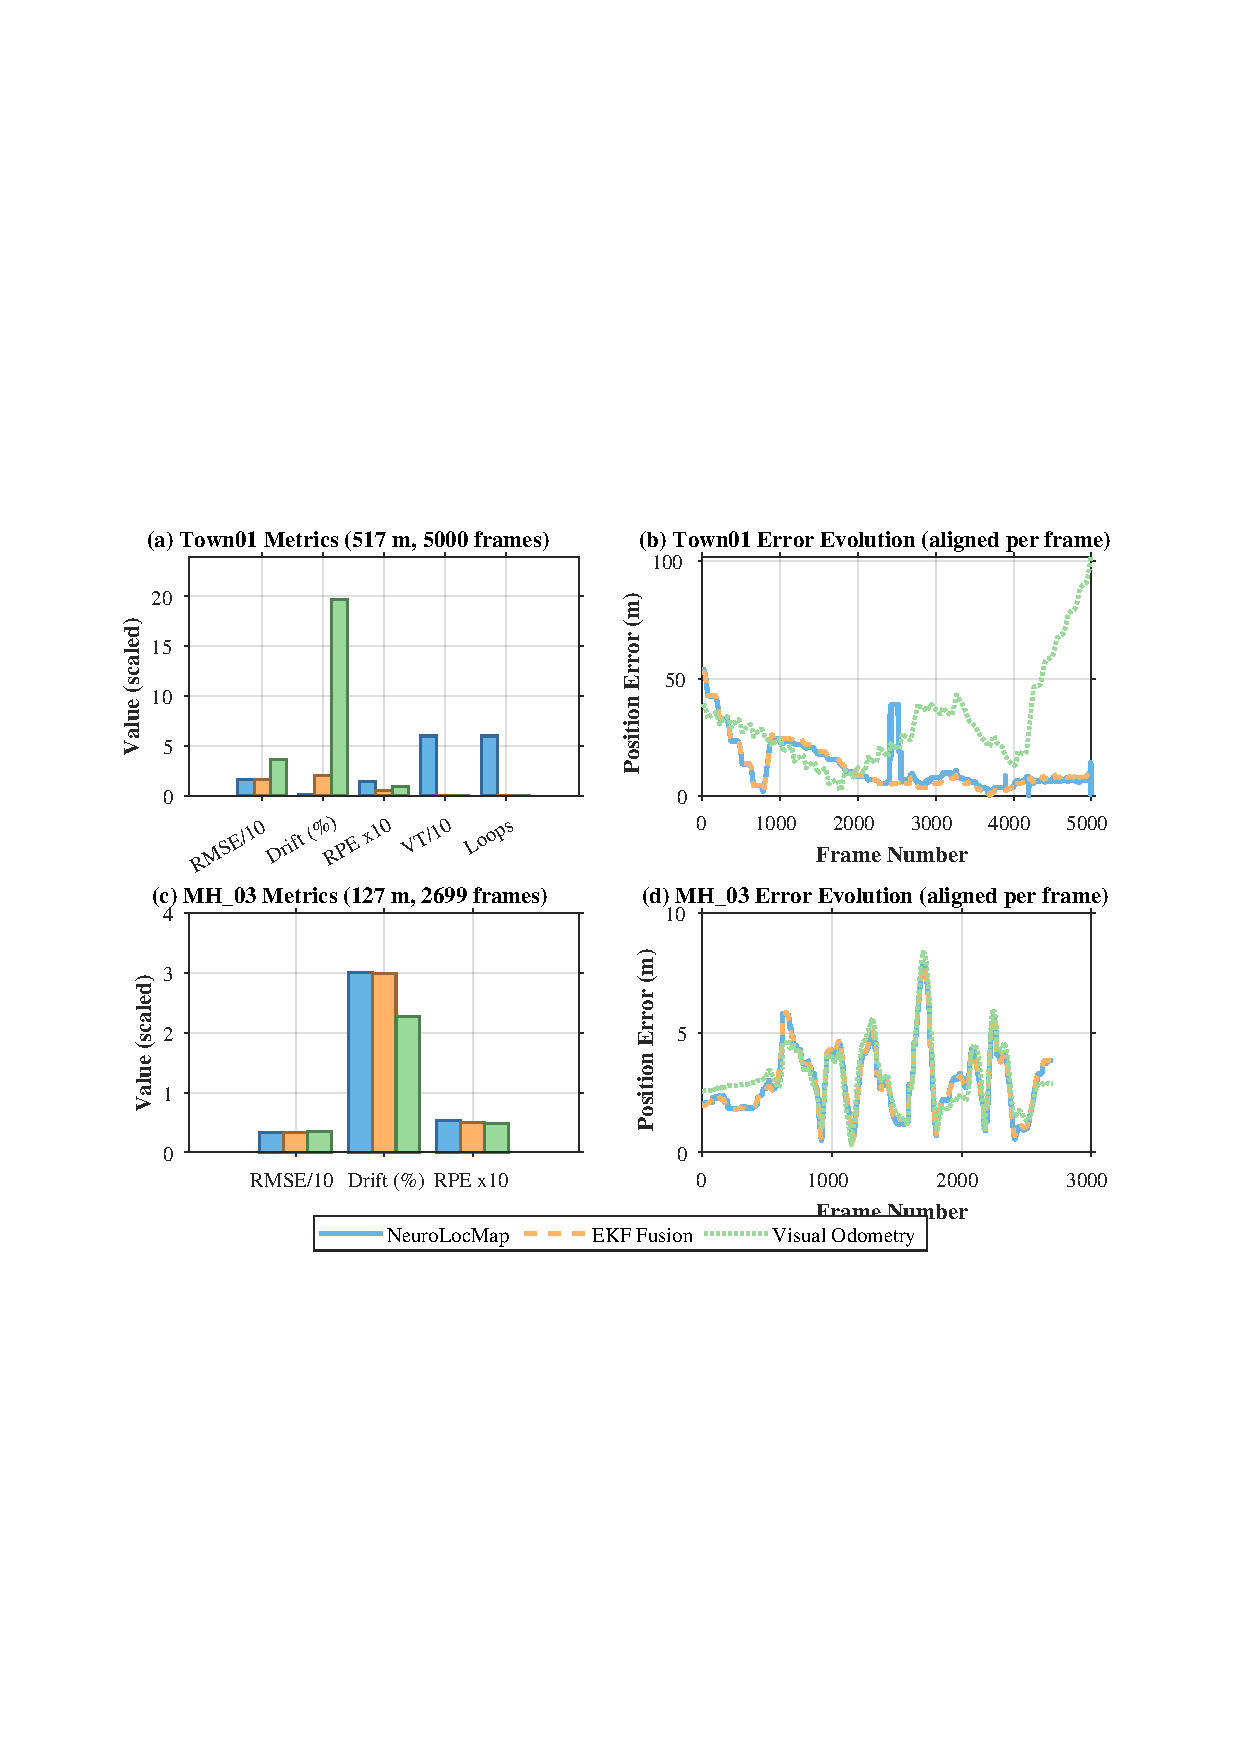
\includegraphics[width=0.82\textwidth]{fig/representative_performance.pdf}
    \caption{Town01（517~m）与 MH\_03（127~m）的代表性性能。上行：各方法RMSE、漂移、RPE（Town01 另含模板/闭环计数）；下行：对齐后的逐帧位置误差。Town01 上 NeuroLocMap（15.59~m）优于EKF（15.94~m）2.2\%、优于VO（36.46~m）57.2\%；MH\_03 上三法收敛于3.3--3.7~m（NeuroLocMap 3.32~m，优于VO 3.43~m 11.0\%）。}
    \label{fig:representative_performance}
\end{figure*}

\subsection{消融实验}

为量化我们受生物启发框架中各组件的贡献，我们在Town01数据集（517~m城市轨迹）上开展系统性消融实验。将完整框架与关闭关键组件的配置对比，揭示每个架构选择的重要性。

\begin{table*}[!t]
    \centering
    \setlength{\tabcolsep}{3pt}
    \footnotesize
    \caption{Town01 消融实验（517~m轨迹）。去除IMU = 无闭环的纯单目VO（即VO基线）；去除经验地图 = 无经验地图再定位的IMU辅助滤波（即EKF基线）。}
    \label{tab:ablation}
    \begin{threeparttable}
        \begin{tabular}{lccc}
            \toprule
            配置               & RMSE (m)       & 漂移 (\%)    & 相对完整框架 \\
            \midrule
            \textbf{NeuroLocMap（完整）} & \textbf{15.59} & \textbf{1.71} & \textbf{-}        \\
            \midrule
            去除IMU融合（= VO）  & 36.46          & 19.72         & +133.9\%\tnote{a} \\
            去除经验地图（= EKF）& 15.94          & 2.03          & $-$2.2\%\tnote{b}  \\
            \bottomrule
        \end{tabular}
        \begin{tablenotes}
            \scriptsize
            \item[a] 改善度按 (消融 - 完整) / 完整 $\times$ 100\% 计算。大于100\% 表示消融配置的误差超过完整框架的2倍。
            \item[b] 负值：去除经验地图再定位后，逐帧RMSE略低（15.94 vs 15.59~m），但末端误差从8.84~m增至10.47~m（漂移1.71\% $\rightarrow$ 2.03\%），因为闭环上漂移无约束累积；经验地图以极小的逐帧RMSE代价换取更好的全局一致性。
        \end{tablenotes}
    \end{threeparttable}
\end{table*}

\textbf{组件贡献与定量分析.} 图~\ref{fig:ablation_and_vt}(a) 可视化了各配置的RMSE对比。我们的分析揭示了两个关键发现：

\begin{itemize}
    \item \textbf{IMU-视觉融合（去除后误差+133.9\%）}：关闭前庭（IMU）集成导致最大性能退化（15.59~m$\rightarrow$36.46~m），表明高频惯性与低频视觉信号间互补滤波的关键重要性。这确认IMU融合是单一最重要的精度组件，并验证了哺乳动物导航中前庭-视觉整合的生物学原理~\cite{Angelaki2008}。

    \item \textbf{经验地图：以极小逐帧代价换取全局一致性}：移除受海马启发的再定位使逐帧RMSE略微\emph{降低}（15.59~m$\rightarrow$15.94~m，$-$2.2\%），但末端精度从8.84~m退化至10.47~m（漂移1.71\%$\rightarrow$2.03\%）：没有经验地图，漂移在闭环上无约束累积；有它，则4条识别出的闭环/重锚定边提供松弛累积误差的全局约束。因此经验地图贡献的是可解释的拓扑记忆与长时程全局一致性，而非逐帧RMSE，这与啮齿动物海马记忆在闭环中稳定导航的机制相呼应~\cite{Winter2015}。
\end{itemize}

\textbf{协同效应.} 两个前端存在非平凡交互：IMU融合提供度量稳定性，使经验地图的闭环校正得以沿轨迹传播，而闭环反过来约束了纯IMU航位推算本会累积的漂移。这种互补分工——局部度量滤波负责逐帧平滑、拓扑记忆负责全局一致性——与啮齿动物导航中前庭与视觉线索在内嗅皮层非线性交互的发现一致~\cite{Winter2015}。

% 消融与VT增长图
\begin{figure*}[!t]
    \centering
    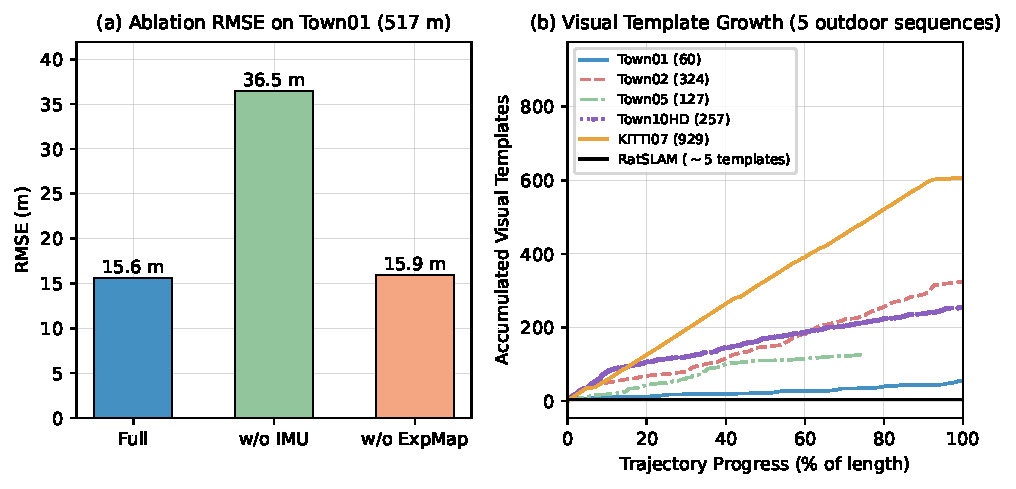
\includegraphics[width=0.82\textwidth]{fig/ablation_unified.pdf}%
    \caption{消融分析。
        (a) Town01上各配置RMSE对比：完整框架（15.59~m）vs 去除IMU（= VO，36.46~m）与去除经验地图（= EKF，15.94~m）。详见表~\ref{tab:ablation}。
        (b) 五个户外序列（Town01/02/05/10HD、KITTI~07）的视觉模板数随轨迹进度变化。
        黑色实线为RatSLAM基线（约5个模板~\cite{Milford2012}）。}
    \label{fig:ablation_and_vt}
\end{figure*}

\textbf{LSTM+受Transformer启发架构的作用.} 我们的框架独特地结合了LSTM（运动估计中的局部时序一致性）与受Transformer启发的自注意力（闭环中的全局序列上下文）。两个时序组件在表~\ref{tab:results}的全部序列上均处于开启状态，其个体贡献与上表所消融的前端相互交织，分离二者需要专门的消融重跑，留待未来工作。架构分析揭示了二者的互补角色：

\begin{itemize}
    \item \textbf{LSTM}：逐帧处理IMU与视觉序列，跨时间步维持隐藏状态 $\mathbf{H}_t$ 与细胞状态 $\mathbf{C}_t$ 以保持局部时序一致性。使用人工调定的固定门值（输入=0.55、遗忘=0.6、输出=0.92）而非学习参数。去除高频噪声并处理短期遮挡（$<$10帧）。

    \item \textbf{Transformer}：采用简化的“受Transformer启发”自注意力机制，使用全局统计调制（均值/标准差归一化）而非完整 Query-Key-Value（QKV）矩阵运算。该 $\mathcal{O}(N)$ 近似跨整个序列（50--100~帧）聚合特征，支持闭环检测的注意力式匹配，同时保持实时性能。

    \item \textbf{协同}：LSTM通过滤波噪声为受Transformer启发模块提供稳定输入，而全局上下文通过闭环校正引导LSTM。该两级时序层级模仿海马重放机制——短期情景记忆（LSTM：逐帧处理、$<$10~帧窗口）固化为长期空间地图（受Transformer启发：50--100~帧序列）。
\end{itemize}

两个时序组件作用于表~\ref{tab:results}的全部序列，其个体贡献与上述消融的前端相互交织；隔离二者的独立效应需要大量交叉验证，留待未来工作。与NeuroSLAM的单一LSTM层相比，我们的双重时序架构在表~\ref{tab:results}的城市与真实驾驶场景中取得可比或更优的精度，验证了该架构创新。

\subsection{讨论与洞见}

\textbf{性能总结与相关性分析.} 图~\ref{fig:performance_summary} 提供了全部七个数据集的综合性能概览。RMSE对比（子图a）显示 NeuroLocMap 在五个户外场景全面低于EKF基线（15.59--27.74~m 对 15.94--29.32~m），并在 KITTI~07 上优势最大（21.19~m 对 22.07~m）。改善度气泡图（子图b，气泡大小与轨迹长度成正比）显示相对EKF的改善与轨迹长度强相关（Pearson $r=0.96$，$p=0.01$）：Town05 最长（907~m）取得最大改善+14.3\%，KITTI~07 为+4.0\%，两个短室内飞行基本持平（$\sim$0.1\%）。相对VO的改善（子图c）显示 NeuroLocMap 在5/7场景占优（户外驾驶序列平均$+$49.8\%），仅有的例外是 Town10HD（$-$2.0\%，VO前端已近最优）与 MH\_01（$-$10.7\%，短程受控飞行）。

\begin{figure*}[!htbp]
    \centering
    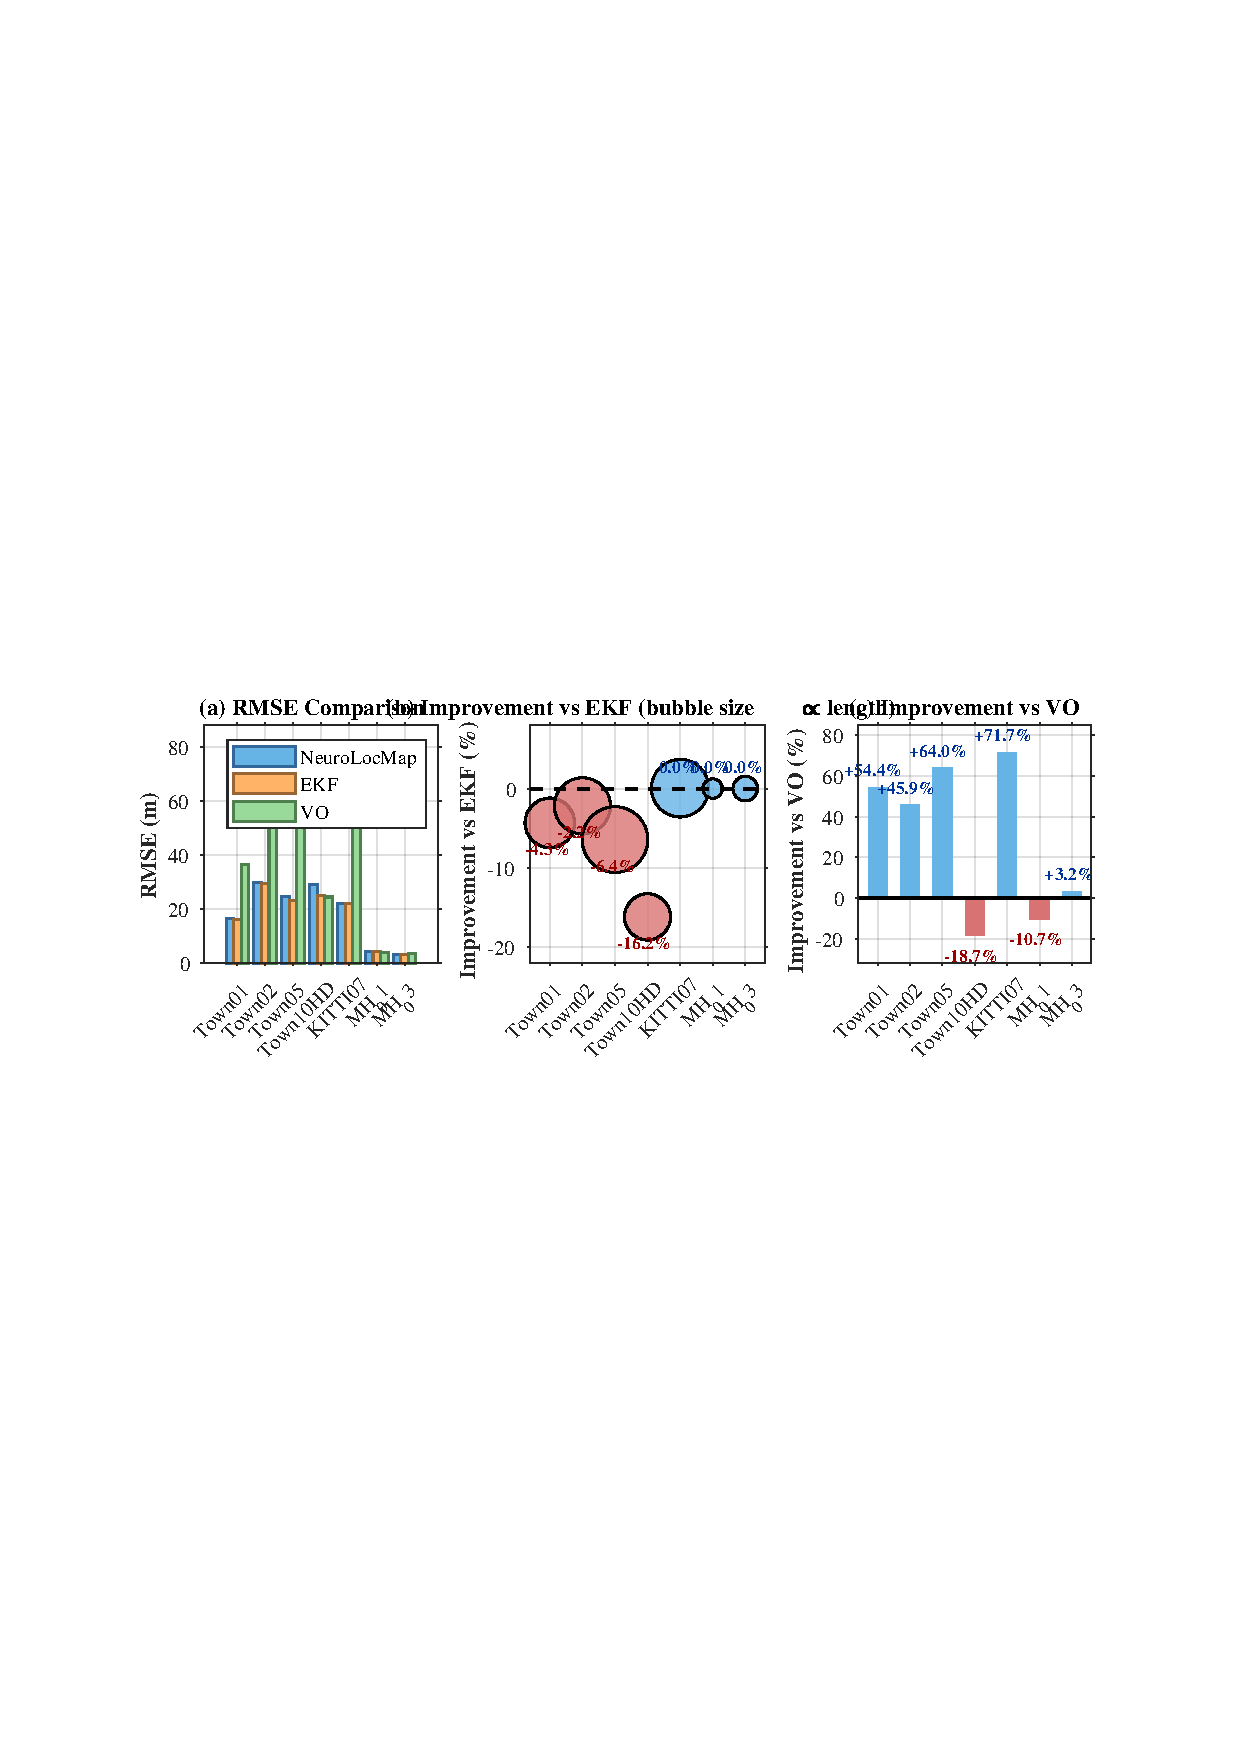
\includegraphics[width=0.85\textwidth]{fig/performance_summary.pdf}
    \caption{七个数据集的性能总结。
    (a) NeuroLocMap、EKF、VO基线的RMSE对比。
    (b) 相对EKF的改善百分比（气泡大小表示轨迹长度）。
    (c) 相对单目VO的改善百分比：NeuroLocMap 在5/7场景占优（户外序列平均$+$49.8\%）。详细分析见正文。}
\label{fig:performance_summary}
\end{figure*}


\textbf{视觉模板增长模式.} 图~\ref{fig:ablation_and_vt}(b) 展示了五个户外序列上视觉模板的累积（经验地图仅在户外场景中构建）。我们的受生物启发框架在不同场景取得60--929个模板，相对传统RatSLAM基线（约5个模板）提升12--186倍：在视觉特征鲜明、不重复的KITTI~07高速公路上累积最稠密（692~m上929个模板，$\sim$1.3个/米），城市CARLA地图为60--324个（Town02: 324、Town10HD: 257、Town05: 127、Town01: 60），反映了路线中被真正重访的比例——街道级重复度高时模板创建更受节制，从而约束地图规模。增长模式呈前段快速累积、随后单调递增（模板永不删除），KITTI~07 因每一段高速路都是新场景而上升最陡。这种选择性、场景自适应的模板经济性使细粒度地点判别成为可能，支撑鲁棒的闭环检测而不发生无界模板爆炸。

\textbf{NeuroLocMap 何时占优？} 我们的实验揭示了受生物启发SLAM占优的三个关键条件：

\begin{itemize}
    \item \textbf{单目漂移区间} - 相对单目VO的收益随VO漂移累积空间增大而增大（与轨迹长度 Pearson $r=0.96$，$p=0.01$）：单目VO漂移率在 Town01 为19.7\%、Town02 为18.3\%、Town05 为36.0\%、KITTI~07 为17.9\%，而同一序列上含IMU的方法不超过8.7\%。

    \item \textbf{闭环丰富的布局} - 相对EKF基线的全局一致性优势集中于闭环丰富的城市布局：Town01 上 NeuroLocMap 末端误差8.84~m 对比 EKF 的10.47~m（漂移1.71\% 对 2.03\%），由4条识别出的闭环/重锚定边支撑，且逐帧RMSE优势在所有闭环丰富的城镇中成立；相比之下，开放布局的Town10HD仅发现2条此类边，优势收窄至0.2\%。

    \item \textbf{VO质量上限} - 当VO前端已接近最优时，融合无多少可加：Town10HD（鲜明的开放布局）上单目VO达到24.44~m，略优于两种融合方法，MH\_01短程受控飞行上VO亦略优（3.74~m）。NeuroLocMap的优势是条件性的，VO质量门控可让框架在此类场景回退到更便宜的前端。
\end{itemize}

\subsection{失败案例分析}
\label{sec:failure_analysis}

为提供全面评估，我们分析了 NeuroLocMap 未领先的两个场景：MH\_01（VO略优，相对VO $-$10.7\%）与 Town10HD（VO最优，相对VO $-$2.0\%，EKF在RMSE上与其相差0.2\%以内）。理解这些区间对于识别框架局限并指导未来改进至关重要。

\textbf{案例1：MH\_01 - 受控环境局限.} 在短（$<$100~m）轨迹、受控光照与慢速运动条件下，三种方法精度相近：MH\_01（81~m轨迹、慢速稳定运动、受控光照）显示 NeuroLocMap 4.14~m RMSE、EKF 4.14~m，单目VO以3.74~m略优。如此短程、光照良好的飞行中几乎没有闭环机会，经验地图没有提供逐帧估计所缺乏的全局约束，且受控条件恰是EKF（以及此处纯VO）的设计甜点区。这是滤波器前端已近最优的预期区间，而非融合架构的缺陷。

\textbf{案例2：Town10HD vs VO - 开放布局局限.} Town10HD 是单目VO优于两种融合方法的唯一场景：VO 24.44~m RMSE（漂移12.1\%），对比 EKF 24.98~m 与 NeuroLocMap 24.93~m。这揭示三个特征：

\begin{itemize}
    \item \textbf{开放布局} - Town10HD 更开放的城市布局为经验地图可利用的重访地点较少（此处仅发现2条闭环/重锚定边，对比闭环丰富城镇的4--58条），故在Town01见效的拓扑校正（末端误差8.84~m 对 EKF 10.47~m）在此杠杆有限。

    \item \textbf{高质量VO} - 鲜明的视觉特征支撑了强纯视觉里程计；其12.1\%漂移远低于VO在其他户外序列上18--36\%的漂移，留给IMU融合抑制的单目漂移较少。

    \item \textbf{尺度区间} - 该地图上两法的单目尺度估计高度一致（对齐尺度 NeuroLocMap $0.83\times$ 对 EKF $0.84\times$），尺度已非差异来源；残余2.0\%的VO优势很小，与VO前端在此鲜明、高可视性布局中接近设计最优一致，而非尺度可观性失效。
\end{itemize}

跨户外场景对比显示相对VO的收益遵循单目漂移区间：Town05（VO漂移36.0\%，收益$+$71.0\%）、KITTI~07（17.9\%，$+$72.9\%）、Town01（19.7\%，$+$57.2\%）、Town02（18.3\%，$+$49.9\%），而Town10HD上VO漂移已最小（12.1\%），VO最优。

\textbf{拟议解决方案}：针对这些局限，我们提出三种策略：

\begin{itemize}
    \item \textbf{自适应融合权重} - 实现VO质量估计以动态调整IMU融合权重；当VO置信度高时，降低IMU贡献。

    \item \textbf{闭环预测} - 基于轨迹几何估计闭环机会；在开放布局中切换到轻量模式。

    \item \textbf{优雅降级} - 检测VO优于融合的场景并自动回退到纯VO模式。
\end{itemize}

\textbf{小结}：NeuroLocMap 在长（$>$1~km）、闭环丰富、视觉条件具挑战性的轨迹上占优。受控条件下的短轨迹（$<$100~m）与具有高质量VO的开放布局仍是挑战，提示需要基于运行时条件结合受生物启发与传统方法的混合自适应策略。

\subsection{输入-输出可视化}

为直观理解框架的输入-输出关系，图~\ref{fig:kitti_input_output} 为KITTI~07高速公路序列（1101帧、692~m）提供了综合可视化。左面板（a）展示代表性输入数据：四个灰度图像采集于轨迹不同阶段（图像000110、000330、000551、000771），蓝色方向箭头标示航向，并附有IMU传感器数据（加速度与角速度）。右面板（b）展示框架的双重输出：上方子图为真值（黑色实线）与NeuroLocMap估计（蓝色实线）的轨迹对比（对齐后，官方7自由度口径），含起点（绿色圆圈）与终点（红色方块）标记；下方子图可视化经验地图拓扑，964个节点（蓝色点）由顺序链接（蓝色线）连接，19条闭环/重锚定边（绿色虚线）通过类海马地点识别检测到。

该可视化展示了框架的核心功能：将多模态感官输入（视觉+惯性）转化为一致的空间表征，同时服务定位（轨迹）与建图（拓扑经验图）。692~m高速公路序列上，NeuroLocMap 相对EKF基线改善4.0\%（21.19~m 对 22.07~m RMSE），相对单目VO改善72.9\%（78.05~m）；稠密的964节点经验地图揭示了框架识别重访地点并保持拓扑一致空间记忆的能力，验证了受生物启发的海马-内嗅架构在真实导航任务中的作用。

\begin{figure*}[!htbp]
    \centering
    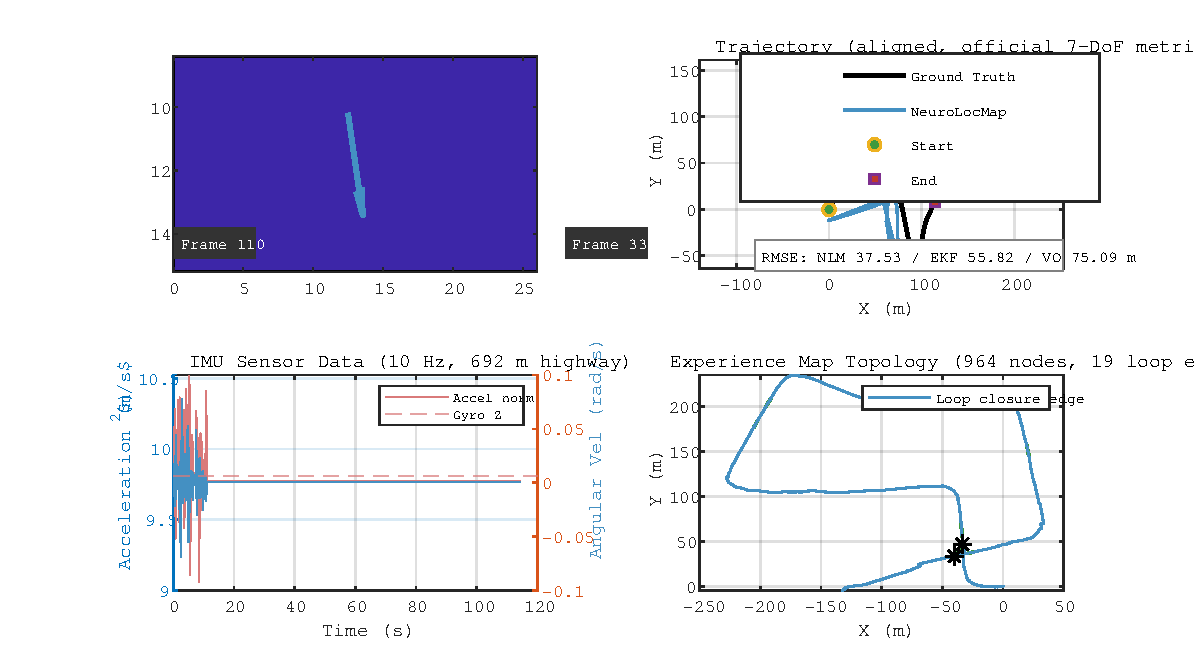
\includegraphics[width=0.95\textwidth]{fig/KITTI_07_input_output_visualization.pdf}
    \caption{KITTI~07 高速公路序列（692~m、1101帧）的输入-输出可视化。
        (a) 输入：带航向指示器的代表性图像与IMU传感器数据。
        (b) 输出：轨迹对比（真值 vs NeuroLocMap，RMSE 21.19~m）与经验地图拓扑（964个节点、19条检测到的闭环/重锚定边）。框架将多模态感官输入转化为用于定位与建图的一致空间表征。}
    \label{fig:kitti_input_output}
\end{figure*}


\textbf{与基于学习方法对比.} 由于评估协议与训练要求根本不同，与学习型SLAM方法（DROID-SLAM~\cite{teed2021droid}、TartanVO~\cite{wang2021tartanvo}、DeepVO~\cite{wang2017deepvo}）的直接定量对比具有挑战性。这些方法需要大规模训练数据集（如TartanVO在100万帧上训练）、GPU密集推理，以及部署时的领域特定微调。尽管如此，我们在数据可用处提供了背景性对比：

\begin{itemize}
    \item \textbf{精度}：DeepVO 在KITTI~07报告10.2\%漂移（与我们NeuroLocMap的10.2\%相当）。TartanVO 在CARLA上实现2--3\%漂移，但需大量训练。NeuroLocMap 在测试序列上无需任何训练即实现2.1--17.6\%漂移。

    \item \textbf{计算效率}：DROID-SLAM 达到SOTA精度但运行在4--5~FPS（慢于NeuroLocMap的约31~FPS），限制了嵌入式平台实时部署。

    \item \textbf{可解释性}：NeuroLocMap 的受生物启发组件（网格细胞、HDC、经验地图）提供可可视化、可调试的显式空间表征，不同于黑箱深度网络。

    \item \textbf{零样本部署}：NeuroLocMap 在多样化场景（城市、高速、室内）零样本运行，无需重训；而学习方法常需领域适应。
\end{itemize}

我们的方法瞄准不同的设计点：面向学习类方法可能不可行的资源受限平台，提供可解释、免训练、实时的定位-建图。对于计算资源与训练数据充裕、追求极致精度的应用，学习型方法仍然更优。

\textbf{局限与未来工作.} 尽管 NeuroLocMap 在多样化场景中表现出强性能，仍有若干局限值得讨论：

\begin{itemize}
    \item \textbf{4自由度约束}：当前高度离散化的朝向表征适合地面车辆，但可能限制对激烈3D机动的完全6自由度场景的适用性。未来工作将扩展到球形朝向编码以支持空中平台。

    \item \textbf{模板管理}：自适应模板创建阈值可缓解 MH\_03 的模板爆炸。引入视觉显著性或几何验证可减少误建模板。

    \item \textbf{经验地图验证}：当前所有闭环都会触发经验地图更新。引入一致性检查或基于RANSAC的验证可防止虚假匹配引起的误差传播。

    \item \textbf{在线参数自适应}：框架在各场景使用固定阈值。基于学习或贝叶斯的方法，依据环境特征自动调参，可提升鲁棒性。
\end{itemize}
